\chapter{OPTIMAL INTERPOLATION TO IMPROVE SATELLITE NOWCASTS WITH DATA}
\label{chap:satoi}

references to other sections

- application
- basic background
- results
- extension kalman filter et

PDF and CDF?

provenance tracking?

\section{Satellite to Irradiance Algorithms}
\subsection{UASIBS}

\subsection{Empirical Model}
- based on suny

- improvments to be made

\section{Parameter Estimation}
\label{sec:paramopt}
Section 6 of \cref{app:satoi} discusses the tuning of OI for a
specific location including the estimation of the parameters
$k,\: l,\: d$ by minimizing the mean-squared error (MSE) of the
analysis over sensors withheld from OI.
To perform this minimization a grid search over the parameters was
performed and the resulting MSE for each set of parameters is shown in
\cref{fig:paramopt}.
This figure clearly shows distinct minima in parameter space for the
UASIBS satllite to irradiance model which indicates that  OI is
sensitive to the choice of parameters.
On the other hand, the lack of distinct minima in parameter space for
the empirical model indicates that a wide range of parameters would
give similar results after performing OI.
If in the future the empirical model is chosen as the background model
for an OI based routine, a more thorough investigation into why OI is
insensitive to these parameters is warranted.

\begin{figure}[p]
\centering
\captionsetup[subfigure]{labelformat=empty}
\subfloat{\hspace{-1em} 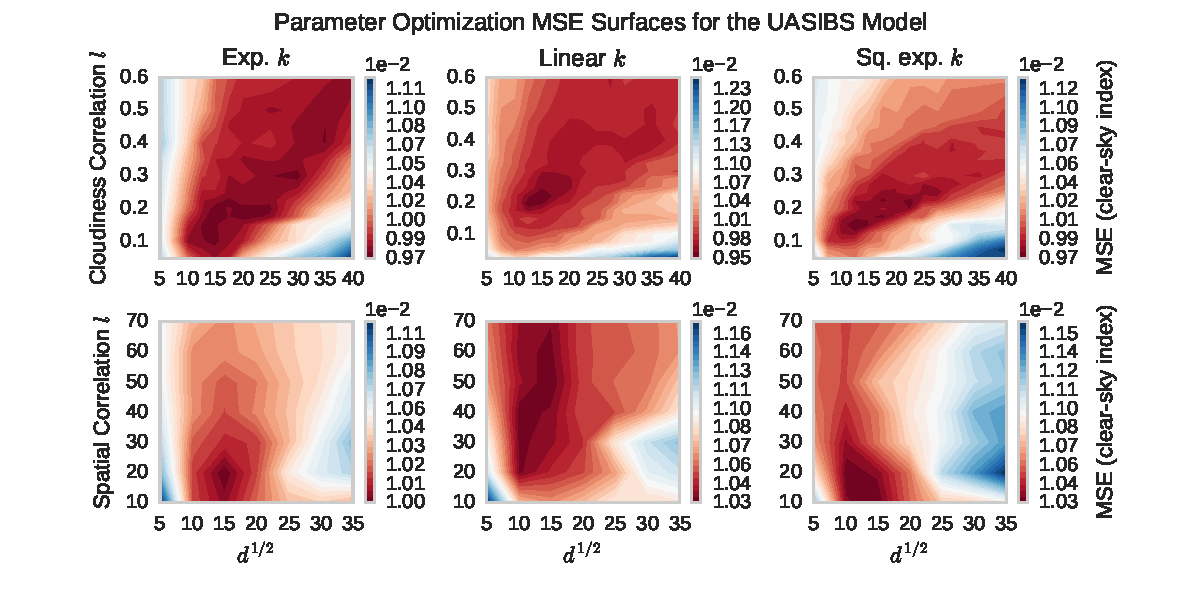
\includegraphics[width=1.05\textwidth]{figs/uasibs_optsurf.pdf}}
\vspace{-1em} \\
\subfloat{\hspace{-1em} 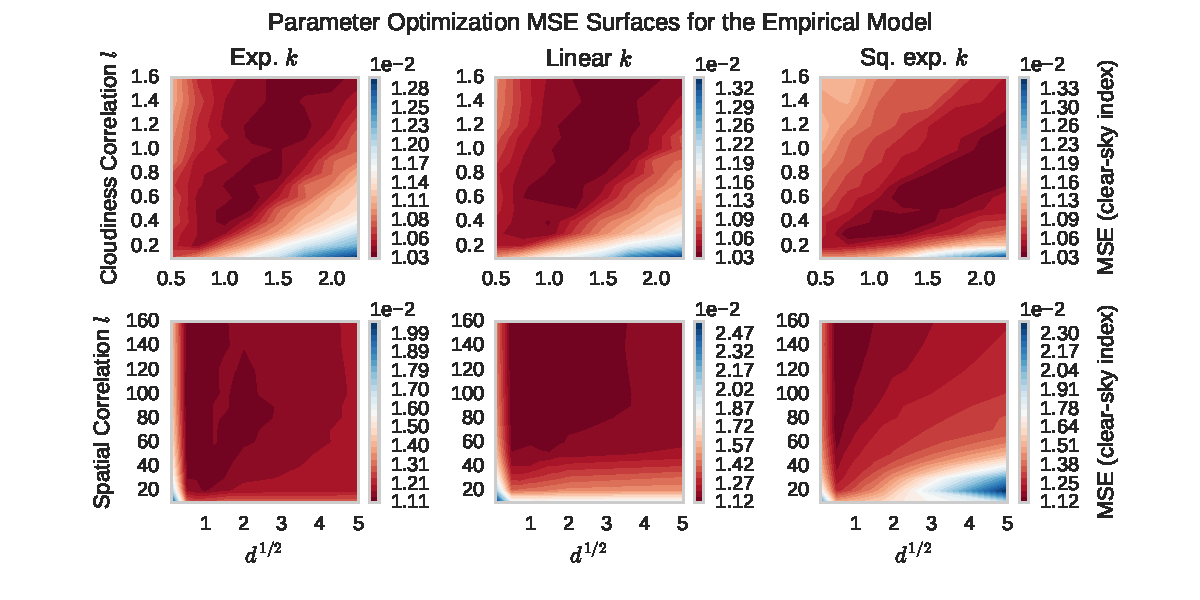
\includegraphics[width=1.05\textwidth]{figs/suny_optsurf.pdf}}
\caption[Optimization surfaces for OI parameters]{Optimization
  surfaces for the parameters $k,\: l,\: d$ of the optimal
  interpolation routine. The columns represent different choices of
  $k$, the rows distinguish between cloudiness and spatial
  correlation, the y-axis is $l$ and the x-axis is $d^{1/2}$. The top
  figure shows surfaces for the UASIBS model and the bottom is for the
  empirical model. Note, that for all choices of $k$ and the
  correlation parameterization, the surfaces for the UASIBS model have
  a clear minimum. The surfaces for the empirical model have less
  distinct minima indicating that optimal interpolation is not
  particularly sensitive to parameter choice for this model.}
\label{fig:paramopt}
\end{figure}


\section{Future Work}
(mainly pertaining to OI, mabye little bit of kalman)

new sat to irr algorithm

Here is some future work

How does NSRDB do?

GSIP?

GOES-16
%%% Local Variables:
%%% mode: latex
%%% TeX-master: "dissertation"
%%% End:
